\section{Pattern utilizzati}

All’interno della classe \texttt{CurrentOperatore.java} sono stati utilizzati due pattern specifici: il \textbf{Singleton} e \textbf{l’Observer}.\\
Il pattern Singleton è utilizzato per garantire che ci sia una sola istanza della classe \texttt{CurrentOperator} nell'applicazione. La classe ha un costruttore privato e un campo statico \texttt{instance}
che rappresenta l'istanza unica della classe. Il metodo \texttt{getInstance()} restituisce l'istanza esistente se è già stata creata o ne crea una nuova se non esiste ancora.
\begin{figure}[H]
    \centering
    \includegraphics[width=1\textwidth]{img/Singleton.png}
    \caption{Costruttore della classe CurrentOperator}
    \label{fig:Singleton}
    
\end{figure}

Questo pattern è stato implementato seguendo questo schema:
\begin{figure}[H]
    \centering
    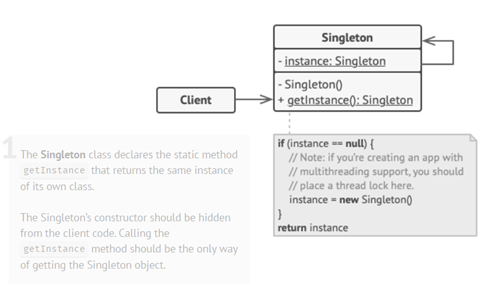
\includegraphics[width=1\textwidth]{img/schema_singleton.png}
    \caption{Schema del pattern Singleton}
    \label{fig:SingletonPattern}
    
\end{figure}

Il pattern Observer è utilizzato per notificare altri oggetti quando l'utente corrente cambia. La classe\texttt{CurrentOperator} definisce un'interfaccia \texttt{CurrentUserChangeListener}
che deve essere implementata da tutte le classi interessate ai cambiamenti dell'utente corrente.
\begin{figure}[H]
    \centering
    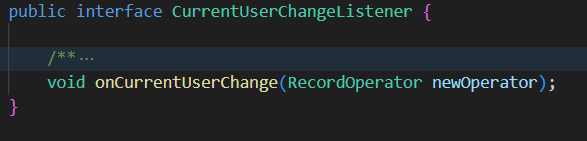
\includegraphics[width=1\textwidth]{img/currentUserChangeListener.png}
    \caption{Interfaccia CurrentUserChangeListener}
    \label{fig:Observer 1}
\end{figure}
La classe contiene metodi per aggiungere (\texttt{addCurrentUserChangeListener}) e rimuovere (\texttt{removeCurrentUserChangeListener}) listener interessati ai cambiamenti dell'utente corrente.
Quando l'utente corrente cambia, il metodo \texttt{notifyCurrentUserChange} viene chiamato per notificare tutti i listener registrati.
\begin{figure}[H]
    \centering
    \includegraphics[width=1\textwidth]{img/notifyCurrentUserChange.png}
    \caption{Metodo notifyCurrentUserChange}
    \label{fig:Observer 2}
\end{figure}
In questo modo, altre parti dell'applicazione possono essere avvisate quando l'utente corrente cambia, consentendo una gestione flessibile degli eventi correlati all'utente.

Questo pattern è stato implementato seguendo questo schema:
\begin{figure}[H]
    \centering
    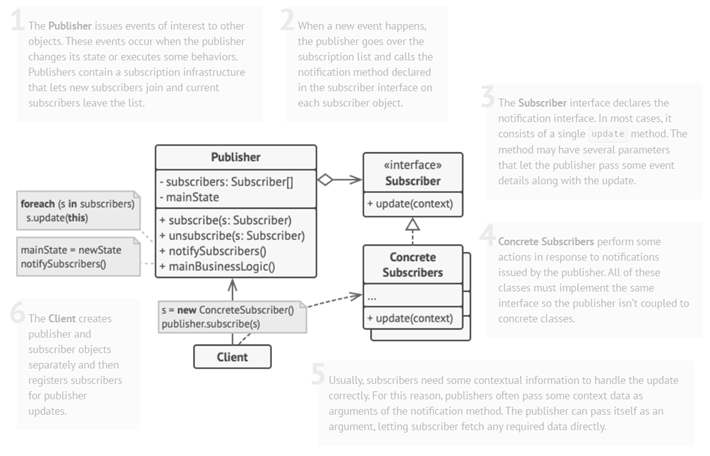
\includegraphics[width=1\textwidth]{img/schema_observer.png}
    \caption{Schema del pattern Observer}
    \label{fig:ObserverPattern}
\end{figure}